\documentclass[border=3pt,varwidth]{standalone}
\usepackage{amsmath,amssymb}
\usepackage{tikz}
\usetikzlibrary{arrows.meta,calc,decorations.markings,patterns,positioning,angles,quotes}
\tikzset{
  >=Stealth,
  every node/.style={font=\normalsize},
  wire/.style={line width=0.9pt},
  thinwire/.style={line width=0.6pt},
  fieldline/.style={line width=0.6pt,-{Stealth[length=2.2mm]}},
  axis/.style={line width=0.7pt,-{Stealth[length=2.2mm]}},
  dashedwire/.style={line width=0.9pt,dash pattern=on 3pt off 2pt},
  resistor/.style={line width=0.9pt},
  chargepos/.style={circle,draw,line width=0.8pt,minimum size=5mm,inner sep=0pt},
  dotcharge/.style={circle,fill,inner sep=0pt,minimum size=2.4pt}
}
% Draw a resistor box centered at (x,y) with width w, height h, horizontal
\newcommand{\resbox}[4]{%
  % #1=x #2=y #3=halfwidth #4=label
  \draw[resistor] (#1-#3,#2-0.18) rectangle (#1+#3,#2+0.18);
  \ifx\\#4\\\else\node[above=2pt] at (#1,#2+0.18) {#4};\fi
}
% Battery symbol: long thin line (+) then short thick line (-), centered at (x,y)
\newcommand{\battery}[2]{%
  % #1=x #2=y ; long line left=+, short line right=- by default orientation
  \draw[wire] (#1-0.09,#2-0.32) -- (#1-0.09,#2+0.32);
  \draw[line width=2.6pt] (#1+0.09,#2-0.16) -- (#1+0.09,#2+0.16);
}

\begin{document}
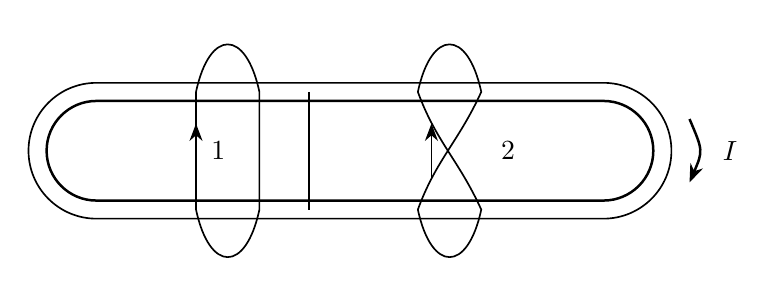
\begin{tikzpicture}[scale=1.15]
  % outer current-carrying wire: stadium/racetrack shape, drawn as a double line
  \draw[wire] (-3.0,0.55) -- (2.6,0.55) arc[start angle=90,end angle=-90,radius=0.55] -- (-3.0,-0.55) arc[start angle=-90,end angle=-270,radius=0.55];
  \draw[thinwire] (-3.0,0.75) -- (2.6,0.75) arc[start angle=90,end angle=-90,radius=0.75] -- (-3.0,-0.75) arc[start angle=-90,end angle=-270,radius=0.75];
  % current direction arrow on the right end of the wire
  \draw[wire,-{Stealth[length=2.3mm]}] (3.55,0.35) .. controls (3.7,0.0) .. (3.55,-0.35);
  \node[right=2pt] at (3.75,0) {$I$};

  % Amperian loop 1: threads the wire zero times -- a loop that bulges above
  % and below the wire WITHOUT separately encircling it (simple non-crossing curve)
  \draw[thinwire] (-1.9,0.65)
    .. controls (-1.75,1.35) and (-1.35,1.35) .. (-1.2,0.65)
    -- (-1.2,-0.65)
    .. controls (-1.35,-1.35) and (-1.75,-1.35) .. (-1.9,-0.65)
    -- cycle;
  \draw[thinwire,-{Stealth[length=2.2mm]}] (-1.9,-0.3) -- (-1.9,0.3);
  \node[right=2pt] at (-1.9,0) {$1$};

  % straight vertical line just to the right of loop 1 (part of the original figure's
  % visual texture -- a second vertical chord with no arrow, purely decorative lead-line)
  \draw[thinwire] (-0.65,0.65) -- (-0.65,-0.65);

  % Amperian loop 2: threads the wire twice -- a figure-eight style curve that
  % crosses itself once while bulging above and below the wire on both sides
  \draw[thinwire]
    (0.55,0.65)
    .. controls (0.7,1.35) and (1.1,1.35) .. (1.25,0.65)
    .. controls (1.0,0.1) and (0.75,-0.1) .. (0.55,-0.65)
    .. controls (0.7,-1.35) and (1.1,-1.35) .. (1.25,-0.65)
    .. controls (1.0,-0.1) and (0.75,0.1) .. (0.55,0.65)
    -- cycle;
  \draw[thinwire,-{Stealth[length=2.2mm]}] (0.7,-0.3) -- (0.7,0.3);
  \node[right=2pt] at (1.3,0) {$2$};
\end{tikzpicture}
\end{document}
